% Extension 1: Cross-Dataset Robustness Slides

\begin{frame}{Extension 1: Background and Purpose}
    \textbf{Hypothesis:} Eigenvector decomposition generalizes across datasets
    
    \vspace{0.5cm}
    \textbf{Test Cases:}
    \begin{itemize}
        \item \textbf{Writer Independence:} MNIST $\leftrightarrow$ EMNIST-Digits
        \item \textbf{Domain Transfer:} MNIST $\rightarrow$ USPS (16$\times$16 $\to$ 28$\times$28)
        \item \textbf{Geometric Semantics:} MNIST $\rightarrow$ EMNIST-Letters
        \begin{itemize}
            \item O $\to$ 0, I $\to$ 1, Z $\to$ 2, S $\to$ 5
        \end{itemize}
    \end{itemize}
    
    \vspace{0.5cm}
    \textbf{Intuition:} Geometric resemblance should lead to similar eigenvectors
    
    \vspace{0.3cm}
    \small
    All models use Center-of-Mass (CoM) normalization to focus on shape geometry
\end{frame}

\begin{frame}{Extension 1: Results - Generalization Works!}
    \begin{columns}
        \column{0.5\textwidth}
        \textbf{Cross-Dataset Accuracy:}
        \begin{itemize}
            \item MNIST $\to$ EMNIST-Digits: \textbf{97.7\%}
            \item EMNIST-Digits $\to$ MNIST: \textbf{97.9\%}
        \end{itemize}
        
        \vspace{0.3cm}
        \textbf{USPS Transfer:}
        \begin{itemize}
            \item Regularized: \textbf{72.3\%}
            \item Baseline: 53.4\%
            \item Improvement: \textbf{+19 pp}
        \end{itemize}
        
        \column{0.5\textwidth}
        \textbf{Letter $\to$ Digit Mapping:}
        \begin{itemize}
            \item O $\to$ 0: \textbf{99.6\%}
            \item I $\to$ 1: \textbf{87.1\%}
            \item Z $\to$ 2: \textbf{88.8\%}
            \item S $\to$ 5: \textbf{87.4\%}
        \end{itemize}
    \end{columns}
\end{frame}

\begin{frame}{Extension 1: Eigenvector Comparison}
    \begin{center}
        \begin{figure}
            \centering
            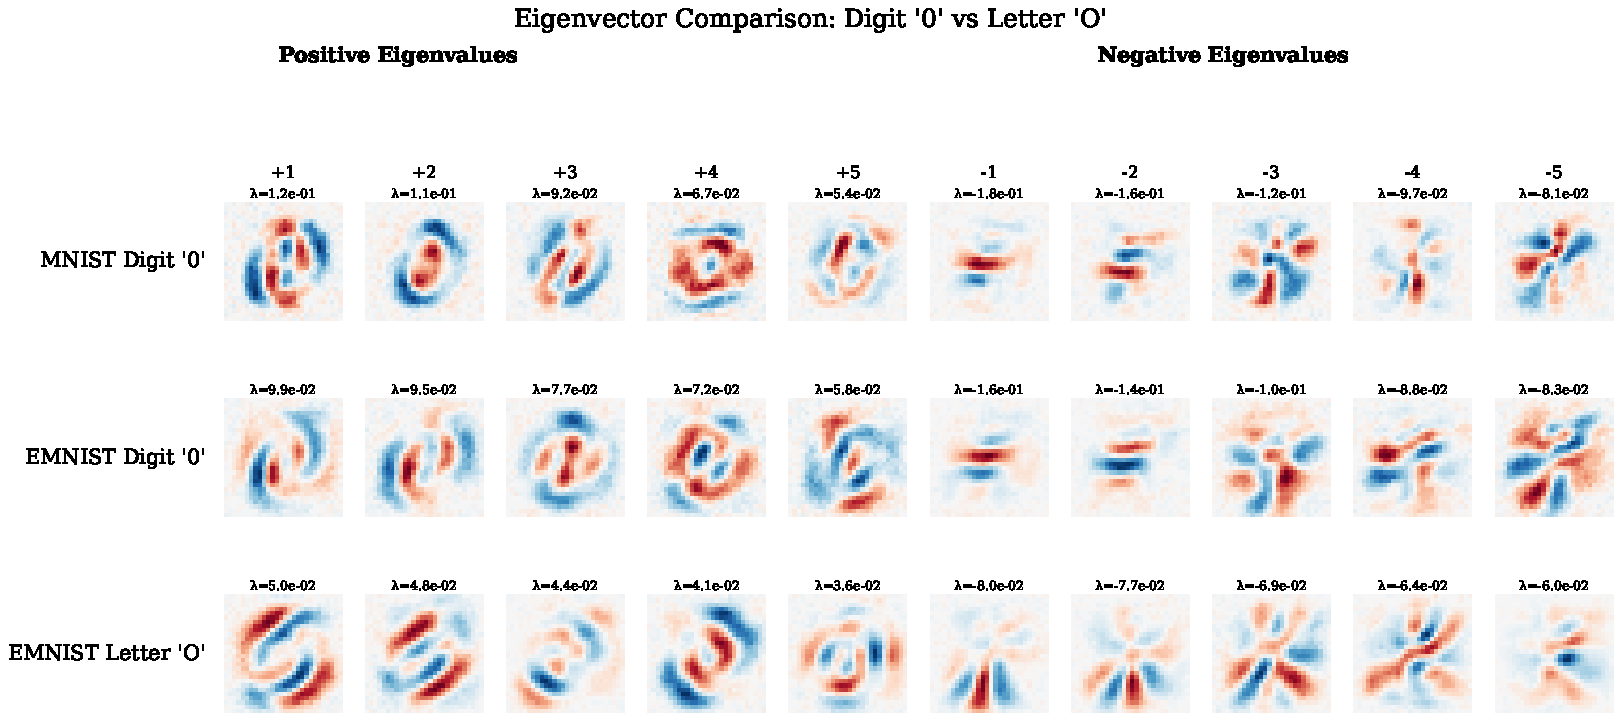
\includegraphics[width=0.9\textwidth]{../Report/figures/extension2/extension2_3way_comparison.pdf}
            \caption{Eigenvector Comparison: Digit '0' vs Letter 'O'}
        \end{figure}
    \end{center}
\end{frame}

\begin{frame}{Quadratic Form Similarity}
    \textbf{Problem:} Cosine similarity fails
    \begin{itemize}
        \item Similar pairs (0--O): 0.358
        \item Dissimilar pairs (0--X): 0.339
        \item Not discriminative!
    \end{itemize}
    
    \vspace{0.5cm}
    \textbf{Solution:} Quadratic Form Similarity
    \begin{equation*}
        \text{sim}(A, B) = \frac{\text{tr}(A \cdot B)}{\|A\|_F \|B\|_F} \in [-1, 1]
    \end{equation*}
    
    \vspace{0.3cm}
    \textbf{Results:}
    \begin{itemize}
        \item Similar pairs: \textbf{0.400}
        \item Dissimilar pairs: \textbf{-0.060}
        \item Large gap with $p < 10^{-4}$
    \end{itemize}
    
    \vspace{0.2cm}
    \small
    Incorporates eigenvalue signs and eigenvector alignment
\end{frame}

\begin{frame}{Extension 1: Quadratic Form Similarity Heatmap}
    \begin{center}
        \begin{figure}
            \centering
            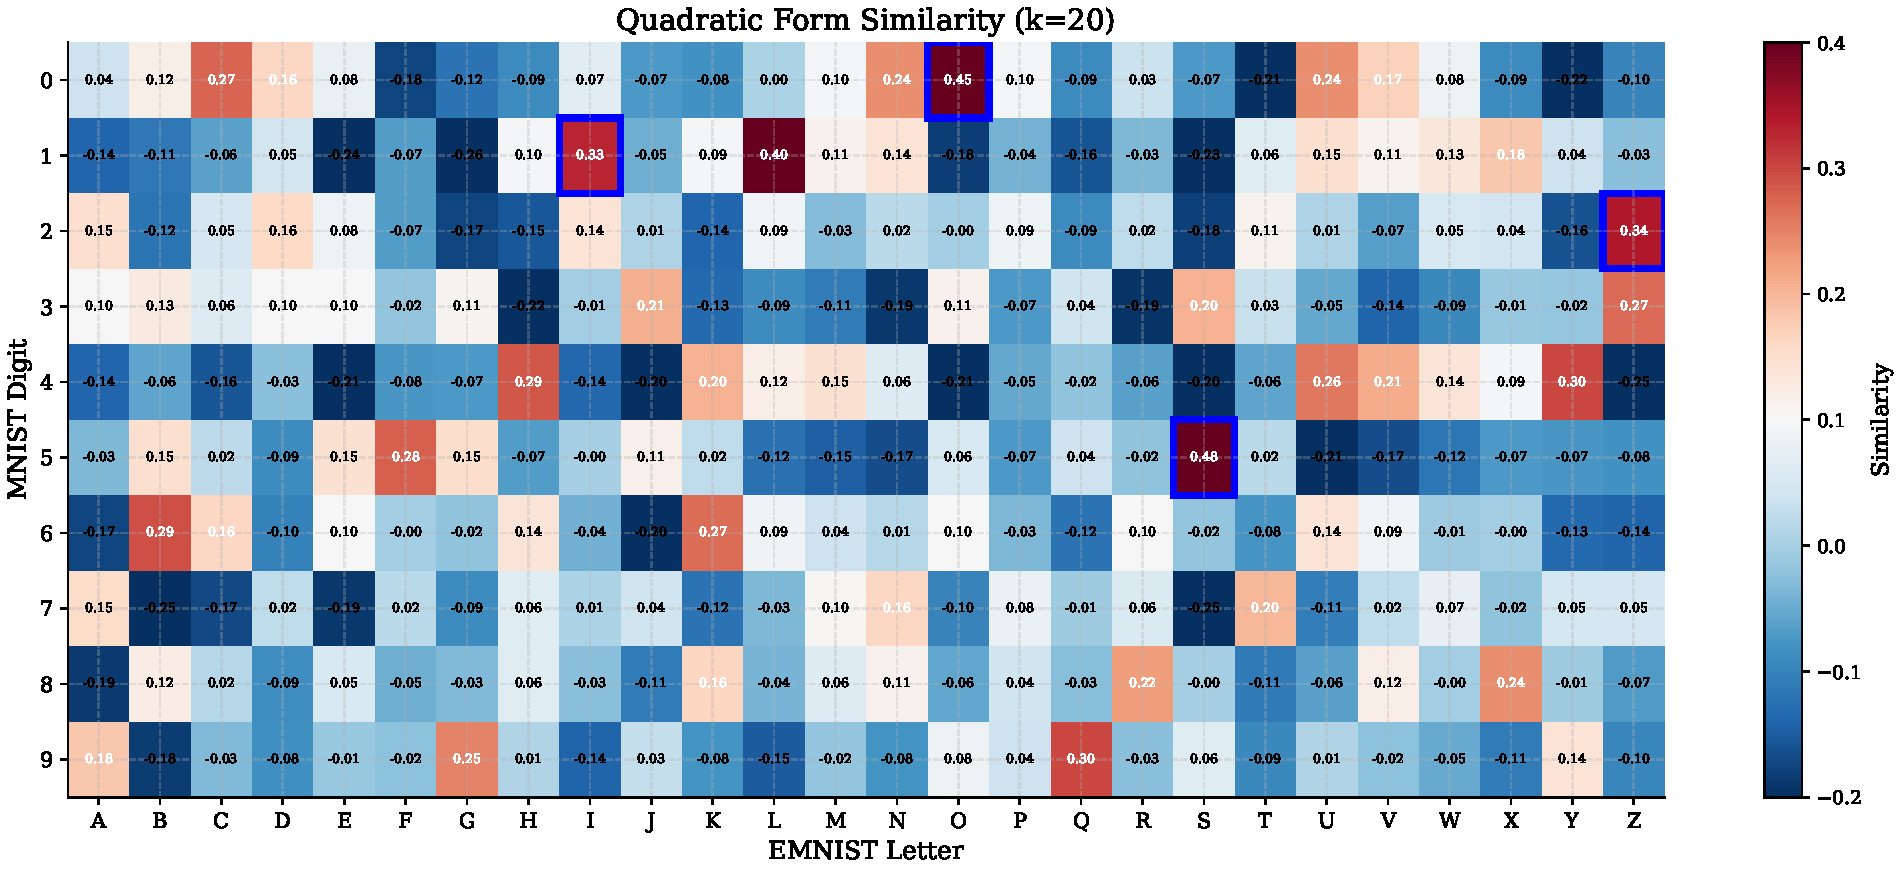
\includegraphics[width=0.85\textwidth]{../Report/figures/extension2/extension2_heatmap_quadratic_form.pdf}
            \caption{Quadratic Form Similarity Heatmap}
        \end{figure}
        \vspace{0.3cm}
        \small
        Clear discrimination: strong diagonal for MNIST vs.\ EMNIST-Digits; bright entries at shape-matched pairs (0--O, 1--I, 2--Z, 5--S)
    \end{center}
\end{frame}

\begin{frame}{Extension 1: Key Figures}
    \begin{columns}
        \column{0.5\textwidth}
        \begin{figure}
            \centering
            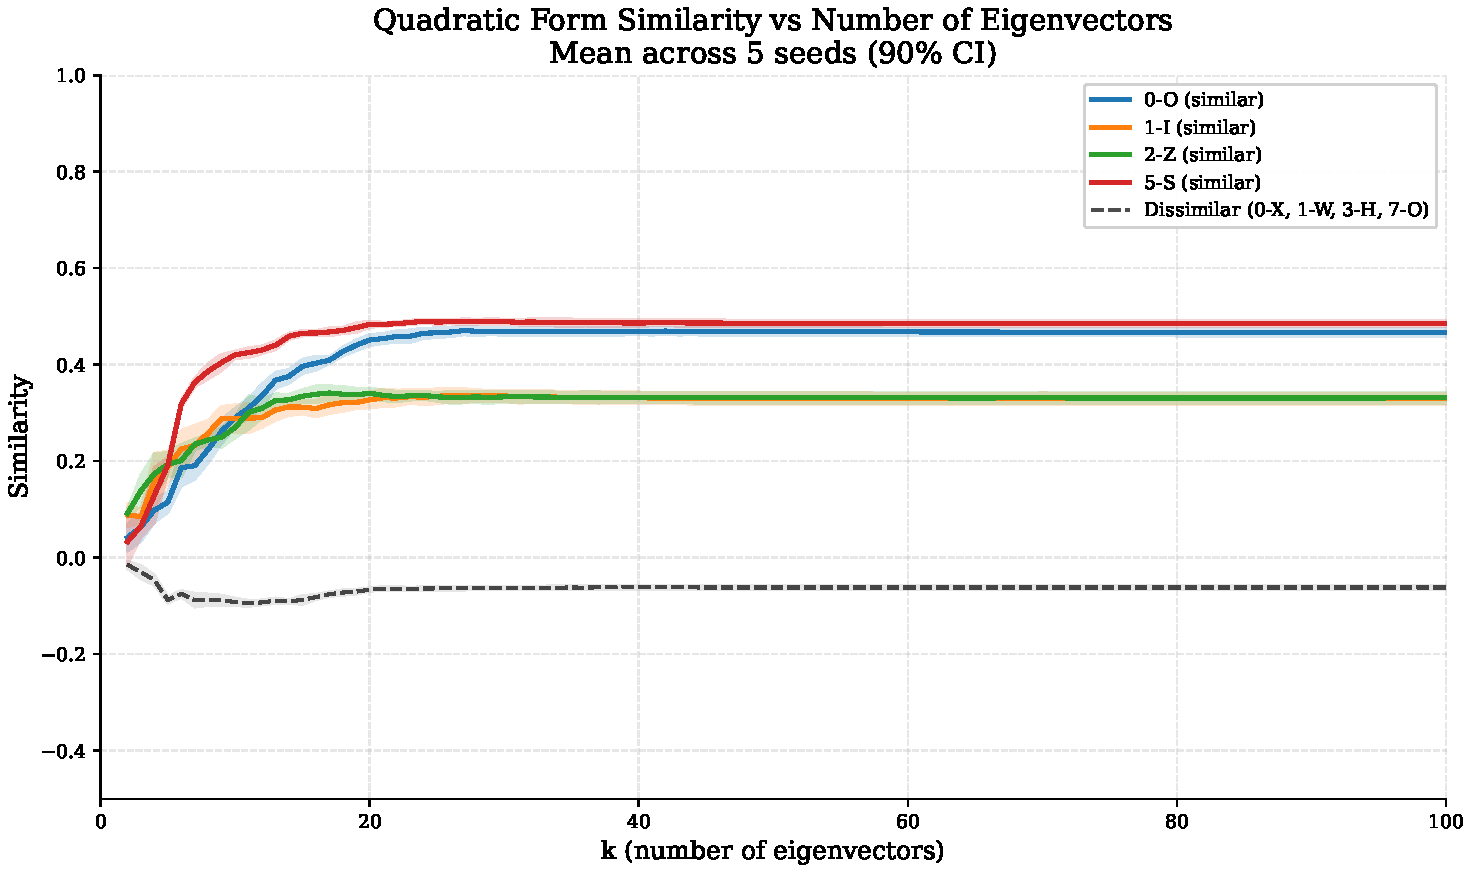
\includegraphics[width=\textwidth]{../Report/figures/extension2/extension2_similarity_vs_k_quadratic_form.pdf}
            \caption{Similarity vs Top-k Eigenvectors}
        \end{figure}
        
        \column{0.5\textwidth}
        \begin{figure}
            \centering
            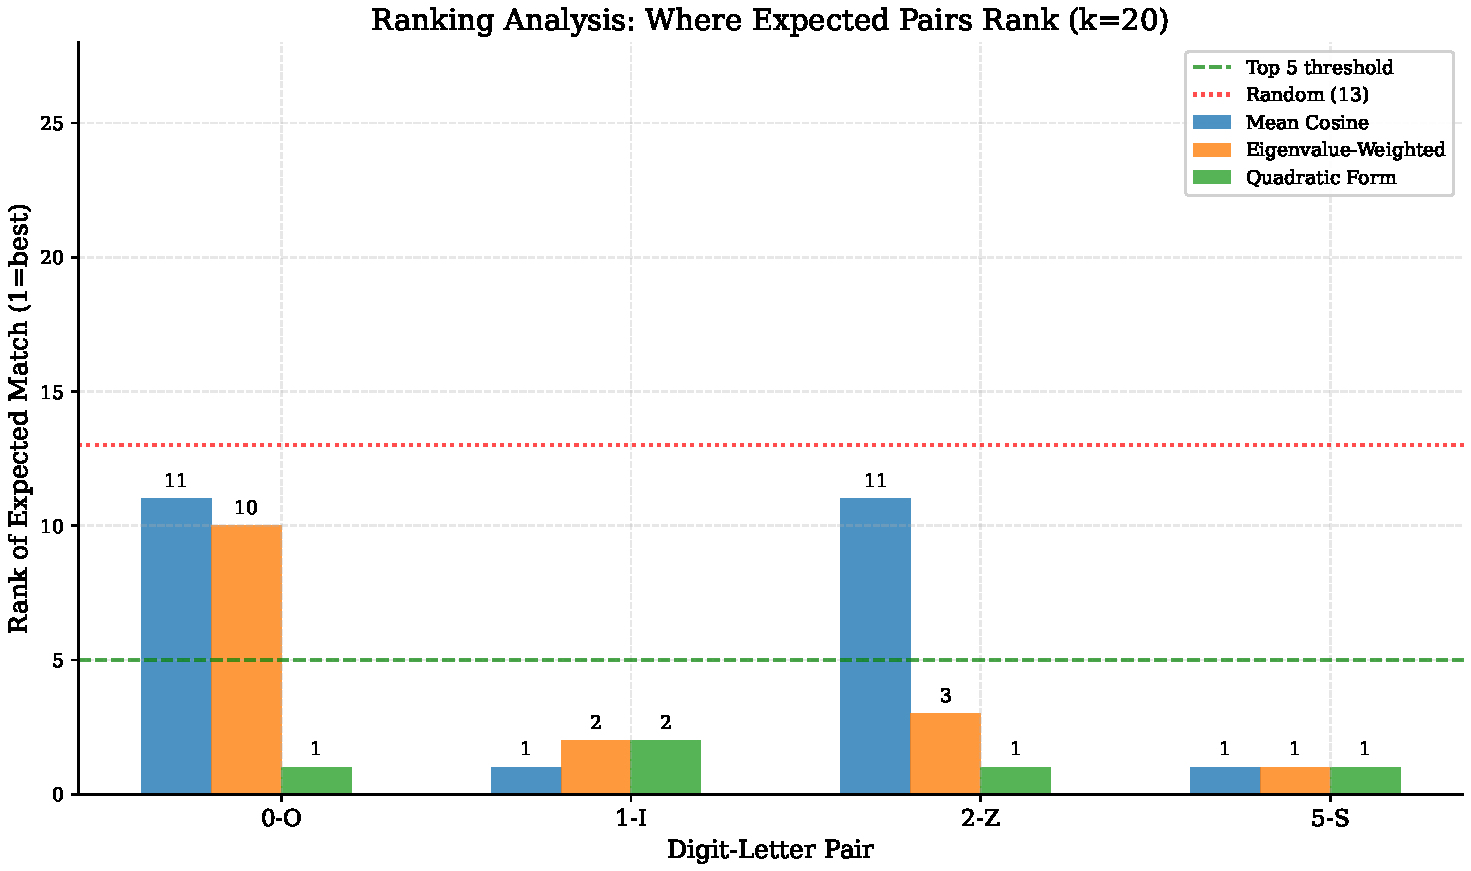
\includegraphics[width=\textwidth]{../Report/figures/extension2/extension2_ranking_analysis.pdf}
            \caption{Ranking Analysis: 3/4 similar pairs rank \#1}
        \end{figure}
    \end{columns}
\end{frame}
